% paperbot_parliament_v3.tex
% pdflatex + mathpazo
% Author: Flyxion (Independent Researcher)

\documentclass[12pt, a4paper]{article}
\usepackage[T1]{fontenc}
\usepackage[utf8]{inputenc}
\usepackage{mathpazo}
\usepackage{microtype}
\usepackage{geometry}
\geometry{margin=1.2in}
\usepackage{setspace}
\onehalfspacing
\usepackage{titlesec}
\usepackage{hyperref}
\hypersetup{colorlinks=true, linkcolor=black, citecolor=black, urlcolor=black}
\usepackage{amsmath, amssymb, amsthm}
\usepackage{listings}
\usepackage{xcolor}
\usepackage{booktabs}
\usepackage{enumitem}
\usepackage{mdframed}
\usepackage{tikz}
\usetikzlibrary{shapes.geometric, arrows.meta, positioning, fit, backgrounds}
\usepackage[ruled, vlined, linesnumbered]{algorithm2e}

% -- theorem environments -----------------------------------------------------

\newtheorem{definition}{Definition}[section]
\newtheorem{proposition}{Proposition}[section]
\newtheorem{corollary}{Corollary}[section]
\newtheoremstyle{principle}{6pt}{6pt}{\itshape}{}{\bfseries}{.}{0.5em}{}
\theoremstyle{principle}
\newtheorem{principle}{Principle}[section]
\theoremstyle{definition}
\newtheorem{conjecture}{Conjecture}[section]

% -- trace box ----------------------------------------------------------------

\newmdenv[
  backgroundcolor=gray!8,
  linecolor=gray!50,
  linewidth=0.5pt,
  innerleftmargin=10pt,
  innerrightmargin=10pt,
  innertopmargin=8pt,
  innerbottommargin=8pt,
]{tracebox}

% -- code listings ------------------------------------------------------------

\definecolor{codebg}{gray}{0.95}
\definecolor{codeframe}{gray}{0.75}
\lstset{
  backgroundcolor=\color{codebg},
  frame=single, framesep=4pt,
  rulecolor=\color{codeframe},
  basicstyle=\ttfamily\small,
  breaklines=true, keepspaces=true,
  columns=fullflexible, captionpos=b,
}

% -- TikZ styles for the pipeline diagram -------------------------------------

\tikzset{
  block/.style={
    rectangle, rounded corners=3pt,
    minimum width=2.6cm, minimum height=0.7cm,
    text centered, font=\small,
    draw=gray!60, fill=white,
  },
  officeblock/.style={
    rectangle, rounded corners=2pt,
    minimum width=2.0cm, minimum height=0.65cm,
    text centered, font=\small\itshape,
    draw=gray!50, fill=gray!8,
  },
  arrow/.style={-Stealth, thick, gray!70},
  thinline/.style={gray!50, thin},
}

% -- section formatting -------------------------------------------------------

\titleformat{\section}{\large\bfseries}{\thesection.}{0.6em}{}
\titleformat{\subsection}{\normalsize\bfseries}{\thesubsection.}{0.5em}{}
\titleformat{\subsubsection}{\normalsize\itshape}{\thesubsubsection.}{0.5em}{}

% -- algorithm2e style --------------------------------------------------------

\SetAlgoLined
\SetKwInput{KwIn}{Input}
\SetKwInput{KwOut}{Output}
\SetKwBlock{ForEach}{for each}{end}
\SetKwFor{ForCyc}{for}{do}{end}
\newcommand{\algcomment}[1]{\tcp*[r]{\footnotesize #1}}

% =============================================================================

\title{\textbf{Paperbot Parliament: A Multi-Agent Framework\\
for Distinction-Centered Document Analysis}\\[0.6em]
\large Concept, Formal Theory, Algorithm, and First Experimental Run}

\author{Flyxion\\
\small Independent Researcher}

\date{\today}

\begin{document}

\maketitle
\newpage

\begin{abstract}
We describe Paperbot Parliament, a multi-agent document analysis system implemented
as a Unix shell pipeline over a local large language model. The system departs from
conventional multi-agent summarization by assigning each agent a constitutionally
distinct analytical role: Claims Extractor, Nitpicker, Skeptic, Archivist,
Synthesist, and Admissibility Auditor. Rather than compressing a document into a
summary, the parliament treats each document chunk as the input to a structured
adversarial process whose primary outputs are distinctions of the form $X \neq Y$.
We develop a formal theory of distinction-centered analysis, introducing the
distinction space $(C, D)$, distinction-preservation score $P$, admissibility
distortion $\mathcal{A}_\pi$, argument admissibility score $\alpha$, and
reconstruction fidelity $F$. We prove a Parliament Stability Theorem showing that
iterated revision cycles are non-increasing in the Lyapunov function
$V(A) = \Delta(A) + \lambda(1 - R)$, and a Parallel Independence Proposition showing
that the architecture structurally prevents recursive summarization collapse. We
report the results of the first experimental run on a theoretical document, in which
29 distinct $X \neq Y$ pairs emerged spontaneously from a single 250-line chunk.
The complete implementation is released as a self-contained Bash script requiring
only Ollama and any locally hosted language model.
\end{abstract}

\newpage
\tableofcontents
\newpage

% =============================================================================
\section{Introduction}
% =============================================================================

The dominant paradigm for automated document analysis is summarization. A summarizer
receives a document and returns a shorter text that preserves the most salient
information according to some implicit measure of salience. The measure is usually
semantic proximity to training data, frequency of term co-occurrence, or position in
the document structure. In each case the output is a compression: a shorter text that
stands in for a longer one.

Compression is useful. It is also dangerous for a specific and rarely articulated
reason. The information destroyed by compression is not uniformly irrelevant.
Compression tends to preserve consensus and discard boundary cases; it tends to
preserve the central tendency of a field and discard the anomalies. Most importantly
for the purposes of the present paper, it tends to preserve facts and discard
distinctions.

A distinction is not a fact. A fact asserts that something is the case:
\emph{Memory involves the hippocampus.} A distinction asserts that two things are
not the same kind of thing: \emph{Memory $\neq$ Storage.} Facts describe what is.
Distinctions describe what must not be confused.

Once this asymmetry is accepted, a cascade of consequences follows. Knowledge
storage becomes distinction preservation. Summarization becomes distinction collapse.
Reasoning becomes navigation between distinctions. And failure becomes the loss of a
distinction that a system could not afford to lose.

The theoretical background for this claim comes from the CLIO framework
(Constraint-Leveraged Inference and Optimization), which holds that the fundamental
unit of intelligence is not the stored fact but the preserved actionable difference.
A system that cannot distinguish reachable futures from stable states, admissible
transitions from reachable states, or prediction accuracy from preservation of
actionable differences, is not merely imprecise---it is incapable of the operations
that depend on those separations.

Paperbot Parliament is an experimental platform for testing whether a structured
multi-agent pipeline can recover distinctions from unstructured text rather than
merely compressing that text into a shorter summary. The answer from the first
experimental run is affirmative: the parliament spontaneously reconstructed a
substantial distinction algebra from a theoretical document without being explicitly
instructed to produce one. The present paper describes the formal theory, the
algorithm, the architecture, the first experimental run, and the theoretical
interpretation of that result.

% =============================================================================
\section{Motivation}
% =============================================================================

\subsection{The Limits of Summarization}

A standard large-language-model summarizer is a function $f : \mathcal{D} \to
\mathcal{D}'$ where $|\mathcal{D}'| \ll |\mathcal{D}|$ under some token-count norm.
The function is trained to maximize agreement between its output and human-produced
summaries of held-out documents. Nothing in this training objective explicitly
preserves distinctions. A summary of a paper that argues $X \neq Y$ may read:
\emph{The paper discusses the relationship between $X$ and $Y$}---semantically
adjacent but representationally catastrophic, because it collapses the very boundary
the paper was written to establish.

This failure mode is not merely a defect of current models that better training will
eventually correct. It is structural. A system optimized to produce text resembling
summaries will converge on whatever features summaries tend to have, and summaries
tend to avoid sharp negations, boundary claims, and ontological separations in favor
of affirmative, encyclopedic prose.

\subsection{Distinctions as Units of Reasoning}

Consider the following pairs extracted from the first Paperbot Parliament run,
reported in Section~\ref{sec:results}:

\begin{quote}
\textsc{distinction}: Memory $\neq$ Storage\\
\textsc{distinction}: Reachability $\neq$ Classification\\
\textsc{distinction}: Health $\neq$ Contents\\
\textsc{distinction}: Failure $\neq$ Temporary Setback\\
\textsc{distinction}: Planning $\neq$ Linear Path\\
\textsc{distinction}: Intelligence $\neq$ Information Processing
\end{quote}

None of these is a fact. Each asserts that two categories which might be conflated
must not be conflated. Each constrains subsequent reasoning by closing off a category
error. A fact tells you what is. A distinction tells you what you must not confuse on
the way to acting.

\subsection{Compression Versus Reconstruction}

The RSVP framework (Relativistic Scalar-Vector Plenum) characterizes a system by a
triple $(\Phi, \mathbf{v}, S)$ of field capacity, transport, and constraint. In this
framework, compression is a reduction in the capacity field $\Phi$ that may or may
not preserve the structure of the constraint surface $S$. The critical question is
not how much information is retained but whether the boundaries in the original
document's concept space survive in the compressed representation.

A multi-agent parliament is one architectural response to this problem. Instead of
applying a single compression function to a document, the parliament applies a set of
analytically distinct functions to the same input, each designed to preserve a
different class of structure. The output is not a shorter document but a richer
analytical artifact that makes visible what a summarizer would have silently discarded.

% =============================================================================
\section{Theoretical Background}
% =============================================================================

\subsection{RSVP: Relativistic Scalar-Vector Plenum}

The RSVP framework models a system as a triple $(\Phi, \mathbf{v}, S)$ where
$\Phi : \mathcal{X} \to \mathbb{R}$ is a scalar capacity field,
$\mathbf{v} : \mathcal{X} \to T\mathcal{X}$ is a transport vector field, and
$S \subseteq \mathcal{X}$ is the constraint surface. A system is healthy to the
extent that many futures remain reachable within the constraint surface. The
health of a system is therefore not a property of its contents but of its future
reachability under its current constraints, yielding: system health $\neq$ system
contents.

\subsection{Admissibility and CLIO}

The admissibility framework distinguishes reachability from admissibility.
Reachability asks: what states are accessible from the current state? Admissibility
asks: which transitions are permitted under the current constraints? These are not the
same question. A state may be reachable via an inadmissible transition, or
unreachable despite being admissible.

CLIO operationalizes admissibility at the representational level. Its central claim
is that a representation should preserve the distinctions relevant to future
admissible action rather than maximizing prediction accuracy. The distinction between
CLIO and standard machine learning is itself a CLIO-type distinction: prediction
accuracy $\neq$ preservation of actionable differences.

\subsection{Repair Theory and Reconstruction}

Repair Theory argues that intelligent systems are not primarily storage systems but
reconstruction systems. Memory retrieval is more accurately described as trajectory
re-entry: the system does not recall a stored object but re-enters a dynamical
trajectory converging on the relevant state. Forgetting is not the loss of stored
information but the loss of reachability of a trajectory. Memory $\neq$ Storage.

A multi-agent parliament is a reconstruction engine for conceptual structure. It does
not store the document; it reconstructs the distinction graph that the document was
written to establish, with each constitutional office following a different analytical
trajectory through the same conceptual space.

% =============================================================================
\section{Formal Theory}
\label{sec:formal}
% =============================================================================

\subsection{Distinction Space}

\begin{definition}[Distinction Space]
Let $C$ be a finite set of concepts occurring in a document corpus. Define a
\emph{distinction relation} $D \subseteq C \times C$ where $(a, b) \in D$ if and
only if the corpus asserts the non-equivalence of $a$ and $b$. The pair
$G_D = (C, D)$ is the \emph{distinction graph} of the corpus.
\end{definition}

The distinction ledger produced by the parliament is a finite approximation to
$G_D$. Each entry \textsc{distinction}: $X \neq Y$ corresponds to a directed edge
$(X, Y) \in D$. The parliament's primary task is: given a document $\mathcal{T}$
with ground-truth distinction graph $G_D^*$, produce an approximation $G_D$
maximizing $|D \cap D^*|$.

\begin{definition}[Distinction-Preservation Score]
Let $D_\mathrm{in}$ be the distinction relation of a source document and
$D_\mathrm{out}$ the distinction relation extracted by an analysis procedure. The
\emph{distinction-preservation score} is
\[
P = \frac{|D_\mathrm{out} \cap D_\mathrm{in}|}{|D_\mathrm{in}|}.
\]
\end{definition}

\begin{definition}[Distinction Entropy]
Let $H_D = \log |D|$ denote the \emph{distinction entropy} of a representation, and
define the \emph{compression factor} $K = H_D^\mathrm{out} / H_D^\mathrm{in}$.
\end{definition}

\begin{principle}[Distinction Preservation]
Two analyses with equal semantic coverage may differ substantially in distinction
entropy. Summary quality $\neq$ distinction quality.
\end{principle}

\subsection{Cumulative Distinction Ledger}

The distinction ledger grows monotonically across chunks. Let $D(C_i)$ denote the
set of $X \neq Y$ pairs extracted from claims $C_i$ of chunk $i$. After $n$ chunks,
the ledger satisfies
\[
L_n = \bigcup_{i=1}^{n} D(C_i),
\]
with the update rule $L_{t+1} = L_t \cup D(C_{t+1})$.

The ledger is therefore not a report but a cumulative approximation to the
corpus-wide distinction graph $G_D$. Each new document contributes new edges to
$(C, L_n)$, and the parliament's cross-session memory is encoded in the growth
of $L_n$ over time.

\subsection{Admissibility Distortion}

\begin{definition}[Admissibility Distortion]
Let $\pi : \mathcal{X} \to \mathcal{M}$ be a projection from conceptual space to
representation space, and let $R(x) \subseteq \mathcal{X}$ denote the reachable
futures from $x$. The \emph{admissibility distortion} of $\pi$ is
\[
\mathcal{A}_\pi =
\frac{\bigl|\{(x_1, x_2) : \pi(x_1) = \pi(x_2),\ R(x_1) \neq R(x_2)\}\bigr|}
{|\mathcal{X}|^2}.
\]
\end{definition}

$\mathcal{A}_\pi$ measures how often $\pi$ collapses two states with different
accessible futures into a single representational point. Summarization is a
projection $\pi_S$ from document-concept space to summary space. The parliament's
purpose, stated precisely, is to minimize $\mathcal{A}_\pi$ rather than
minimize $|\mathcal{M}|$.

\subsection{Argument Admissibility}

\begin{definition}[Argument Admissibility Score]
Let $A = (V, E)$ be a directed graph where vertices $V$ are claims and edges $E$
are inferential steps. Let $B \subseteq E$ be the set of missing bridges detected
by the Auditor. The \emph{argument admissibility score} is
\[
\alpha = 1 - \frac{|B|}{|E|}.
\]
\end{definition}

When $\alpha = 1$, every inferential step is bridged and the argument is fully
admissible. When $\alpha = 0$, every step contains an unresolved gap. The
Auditor's constitutional role is to estimate $|B|$, providing a lower bound on
$1 - \alpha$.

\subsection{Reconstruction Fidelity}

\begin{definition}[Reconstruction Fidelity]
Let $T$ be the conceptual trajectory of a document, $S(T)$ a conventional summary,
and $P(T) = \{N, Sk, Ar, Sy, Au\}(C)$ the parliament's analytical family.
Let $R(\cdot)$ be a reconstruction operator. The \emph{reconstruction fidelity}
of a procedure $Q$ is
\[
F(Q(T)) = \frac{|R(Q(T)) \cap T|}{|T|}.
\]
\end{definition}

\begin{conjecture}[Parliament Reconstruction Advantage]
\label{conj:reconstruction}
For theoretical documents whose primary conceptual content consists of distinctions,
\[
F(P(T)) > F(S(T)).
\]
\end{conjecture}

We distinguish Conjecture~\ref{conj:reconstruction} from the proved results that
follow. The conjecture requires a formal reconstruction operator $R$ and an empirical
comparison across a held-out corpus, outlined in Section~\ref{sec:future}. The first
experimental run provides qualitative evidence in its favor.

\subsection{Revision Fixed Point}

When revision cycles are active, the Revision Office computes
\[
C_{t+1} = R\bigl(C_t,\; N(C_t),\; Sk(C_t),\; Au(C_t)\bigr),
\]
where $N$, $Sk$, $Au$ are the Nitpicker, Skeptic, and Auditor transforms
respectively. This is a fixed-point iteration on the claim set. Each cycle feeds
structural, evidential, and inferential defects back into a repaired claims file,
so the parliament converges toward a claim set that has survived all three
critical offices.

\subsection{Lyapunov Stability}

\begin{definition}[Parliament Lyapunov Function]
Let $\mathrm{pass}(A)$, $\mathrm{fail}(A)$, $\mathrm{rev}(A)$ be the per-verdict
claim counts, $n(A)$ their sum. Define
\[
\Delta(A) = \frac{\mathrm{fail}(A) + \mathrm{rev}(A)}{n(A)},\quad
R(A) = \frac{\mathrm{pass}(A)}{n(A)},\quad
V(A) = \Delta(A) + \lambda(1 - R(A)),\quad \lambda > 0.
\]
\end{definition}

\begin{proposition}[Parliament Stability]
\label{prop:stability}
If every revision cycle (a) removes at least one claim with an unresolved
admissibility violation and (b) introduces no new admissibility violations,
then $V(A_{t+1}) \leq V(A_t)$ for all $t$.
\end{proposition}

\begin{proof}
By (a), $\mathrm{fail}(A_{t+1}) + \mathrm{rev}(A_{t+1})
\leq \mathrm{fail}(A_t) + \mathrm{rev}(A_t) - 1$,
so $\Delta(A_{t+1}) \leq \Delta(A_t)$.
By (b), no new failures are introduced, giving
$R(A_{t+1}) \geq R(A_t)$ and thus
$\lambda(1 - R(A_{t+1})) \leq \lambda(1 - R(A_t))$.
Therefore
\[
V(A_{t+1}) = \Delta(A_{t+1}) + \lambda(1 - R(A_{t+1}))
           \leq \Delta(A_t) + \lambda(1 - R(A_t)) = V(A_t). \qedhere
\]
\end{proof}

\begin{corollary}[Parliament Convergence]
Under the conditions of Proposition~\ref{prop:stability}, the revision cycle
converges to a fixed point $A^*$ at which $\Delta(A^*) = 0$ and $R(A^*) = 1$.
\end{corollary}

% =============================================================================
\section{Algorithm and Architecture}
% =============================================================================

\subsection{Parliament Algorithm}

Algorithm~\ref{alg:parliament} gives the complete procedure. It serves as the
authoritative behavioural specification; the Bash implementation is a faithful
rendering of this pseudocode over standard Unix text streams.

\begin{algorithm}[t]
\caption{Paperbot Parliament}
\label{alg:parliament}
\KwIn{Document $D$; number of revision cycles $c \geq 1$; model $M$}
\KwOut{Parliament report $\mathcal{R}$; distinction ledger $L$}
\BlankLine
$\mathit{Chunks} \leftarrow \mathrm{Split}(D, \ell)$
\algcomment{$\ell = 250$ lines by default}\;
\BlankLine
\ForEach{$\mathit{chunk} \in \mathit{Chunks}$}{
  $C \leftarrow \mathrm{ExtractClaims}(\mathit{chunk}, M)$
  \algcomment{structured claims, definitions, assumptions}\;
  $L \leftarrow L \cup D(C)$
  \algcomment{update cumulative distinction ledger}\;
  \BlankLine
  \ForCyc{$t = 1$ \KwTo $c$}{
    $N  \leftarrow \mathrm{Nitpicker}(C, M)$
    \algcomment{ambiguities, undefined terms, category errors}\;
    $Sk \leftarrow \mathrm{Skeptic}(C, M)$
    \algcomment{unsupported claims, strongest objections}\;
    $Ar \leftarrow \mathrm{Archivist}(C, M)$
    \algcomment{precedents, lineage, missing citations}\;
    $Sy \leftarrow \mathrm{Synthesist}(C, M)$
    \algcomment{patterns, bridges, unification}\;
    $Au \leftarrow \mathrm{Auditor}(C, M)$
    \algcomment{inferential gaps, inadmissible jumps}\;
    \BlankLine
    \If{$c > 1$ \textbf{and} $t < c$}{
      $V \leftarrow \mathrm{Vote}(N, Sk, Ar, Au)$
      \algcomment{per-claim PASS / FAIL / NEEDS\_REVISION}\;
      $C \leftarrow \mathrm{Revise}(C, N, Sk, Au)$
      \algcomment{remove violations, flag needs-evidence}\;
    }
  }
  \BlankLine
  $\mathrm{Archive}(C,\; N,\; Sk,\; Ar,\; Sy,\; Au)$\;
  $\mathcal{R} \leftarrow \mathcal{R} \cup \mathrm{AssembleReport}(\mathit{chunk})$\;
}
\Return $(\mathcal{R},\; L)$\;
\end{algorithm}

The parliament operator for a single chunk with claims $C$ is:
\[
\mathcal{P}(C) = \bigl\{N(C),\; Sk(C),\; Ar(C),\; Sy(C),\; Au(C)\bigr\}.
\]
This set-valued form distinguishes the parliament from a composed pipeline.

\subsection{Parallel Independence and Anti-Collapse}

The central structural property of the algorithm is that all offices receive
identical input.

\begin{proposition}[Parallel Independence]
\label{prop:independence}
If every office $B_i$ receives the same claims file $C$ and no office receives
another office's output, then recursive summarization collapse cannot occur within
a single cycle.
\end{proposition}

\begin{proof}
Each office computes $B_i(C)$ from the shared source $C$. No office computes
$B_i(B_j(C))$ for $i \neq j$. Therefore the composition
$B_n(\cdots(B_2(B_1(C)))\cdots)$, which is the recursive structure responsible
for collapse, never arises. Instead the parliament produces the independent family
$\{B_1(C), B_2(C), \ldots, B_n(C)\}$, in which information loss does not compound
across offices. \qed
\end{proof}

The distinction between $B_n \circ \cdots \circ B_1(C)$ (recursive compression)
and $\{B_i(C)\}$ (parallel family) is the single most important structural property
of the architecture, and it explains the empirical observation that the six office
outputs remained analytically differentiated in the first run.

\subsection{Pipeline Diagram}

Figure~\ref{fig:pipeline} gives the activity diagram of the parliament pipeline.

\begin{figure}[h]
\centering
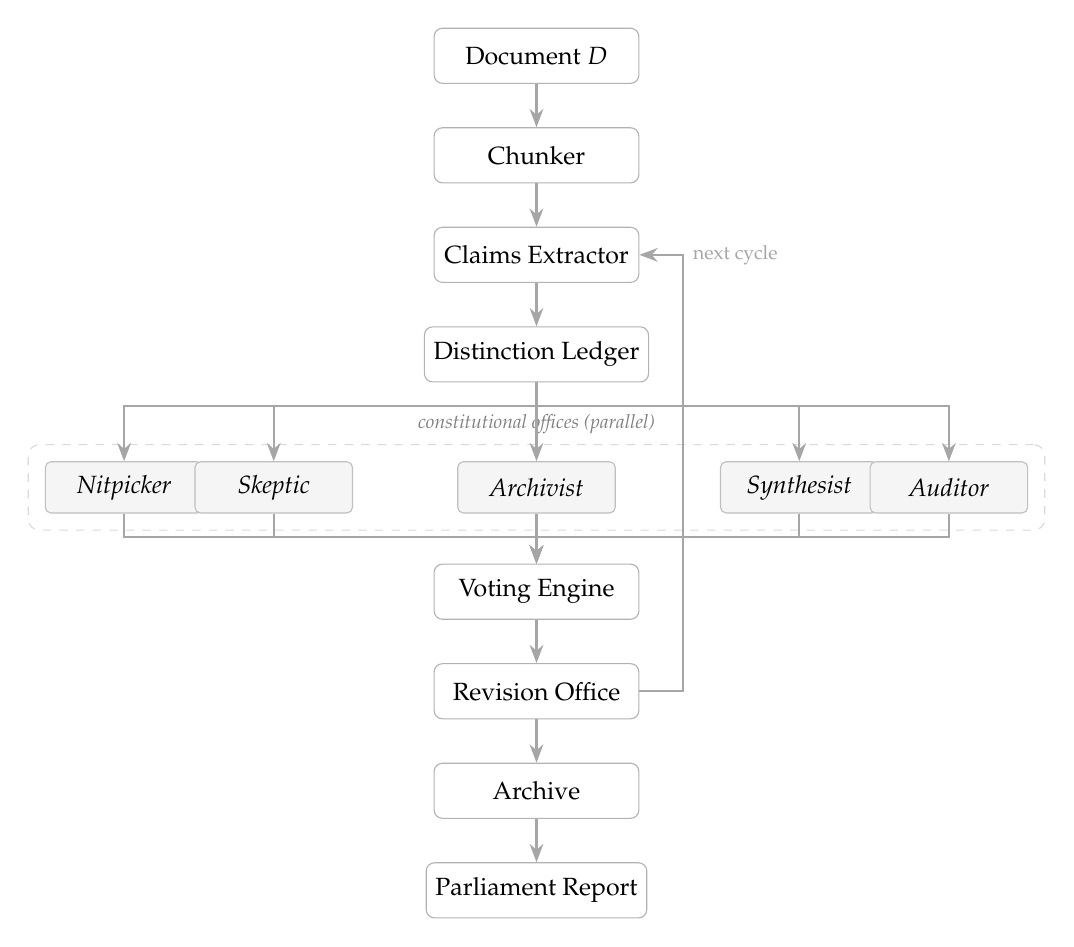
\begin{tikzpicture}[node distance=0.55cm and 1.3cm]

% Main vertical column
\node[block] (doc)     {Document $D$};
\node[block, below=of doc]  (split)   {Chunker};
\node[block, below=of split] (claims) {Claims Extractor};
\node[block, below=of claims] (ledger) {Distinction Ledger};

% Fan out to five offices
\node[officeblock, below left=1.0cm and 2.8cm of ledger]  (nit) {Nitpicker};
\node[officeblock, below left=1.0cm and 0.9cm of ledger]  (sk)  {Skeptic};
\node[officeblock, below=1.0cm of ledger]                  (ar)  {Archivist};
\node[officeblock, below right=1.0cm and 0.9cm of ledger] (sy)  {Synthesist};
\node[officeblock, below right=1.0cm and 2.8cm of ledger] (au)  {Auditor};

% Merge below offices
\node[block, below=2.3cm of ledger] (vote) {Voting Engine};

% Revision and archive
\node[block, below=0.55cm of vote]  (rev)  {Revision Office};
\node[block, below=0.55cm of rev]   (arch) {Archive};
\node[block, below=0.55cm of arch]  (rep)  {Parliament Report};

% Vertical arrows
\draw[arrow] (doc)    -- (split);
\draw[arrow] (split)  -- (claims);
\draw[arrow] (claims) -- (ledger);

% Fan arrows from ledger to offices
\draw[arrow] (ledger.south) -- ++(0,-0.3) -| (nit.north);
\draw[arrow] (ledger.south) -- ++(0,-0.3) -| (sk.north);
\draw[arrow] (ledger.south) -- ++(0,-0.3) -- (ar.north);
\draw[arrow] (ledger.south) -- ++(0,-0.3) -| (sy.north);
\draw[arrow] (ledger.south) -- ++(0,-0.3) -| (au.north);

% Fan back to vote
\draw[arrow] (nit.south) -- ++(0,-0.3) -| (vote.north);
\draw[arrow] (sk.south)  -- ++(0,-0.3) -| (vote.north);
\draw[arrow] (ar.south)  -- ++(0,-0.3) -- (vote.north);
\draw[arrow] (sy.south)  -- ++(0,-0.3) -| (vote.north);
\draw[arrow] (au.south)  -- ++(0,-0.3) -| (vote.north);

\draw[arrow] (vote) -- (rev);
\draw[arrow] (rev)  -- (arch);
\draw[arrow] (arch) -- (rep);

% Revision loop back to claims
\draw[arrow] (rev.east) -- ++(0.55,0) |- node[right, font=\scriptsize] {next cycle} (claims.east);

% Background box around offices
\begin{scope}[on background layer]
  \node[fit=(nit)(sk)(ar)(sy)(au),
        draw=gray!30, dashed, rounded corners=4pt,
        inner sep=6pt,
        label={[font=\scriptsize\itshape, gray]above:constitutional offices (parallel)}] {};
\end{scope}

\end{tikzpicture}
\caption{Activity diagram of the Paperbot Parliament pipeline. The five
constitutional offices operate in parallel on the same claims file, producing
the independent family $\mathcal{P}(C) = \{N(C), Sk(C), Ar(C), Sy(C), Au(C)\}$
rather than a recursive composition. The revision loop is active only when
$c > 1$.}
\label{fig:pipeline}
\end{figure}

\subsection{Complexity Analysis}

For a document with $n$ chunks, $k = 5$ constitutional offices, and $c$ revision
cycles, the number of model invocations per chunk is:
\begin{center}
\begin{tabular}{lr}
Claims Extractor & $1$ \\
Ledger extraction & $1$ \\
Office calls per cycle & $k \cdot c$ \\
Revision passes & $c - 1$ \\
\end{tabular}
\end{center}
giving a total of $M = n(kc + c + 1)$ invocations across the document. For the
default configuration $k = 5$, $c = 1$:
\[
M = n(5 \cdot 1 + 1 + 1) = 7n.
\]
For the first experimental run with $n = 3$ chunks and $c = 1$:
\[
M = 7 \times 3 = 21 \text{ invocations},
\]
consistent with the six office outputs observed for \texttt{chunk\_aa} plus the
claims extractor. Because all offices are data-independent given $C$, the
architecture is embarrassingly parallel: all five office calls within a cycle can
in principle run concurrently, reducing wall-clock time to
$O(n \cdot c)$ invocations on a parallel executor.

\subsection{Unix Pipeline Lineage}

The implementation uses only standard Unix utilities: \texttt{split},
\texttt{cat}, \texttt{grep}, \texttt{awk}, \texttt{tail}, and
\texttt{inotifywait}. It is 682 lines of Bash with a 187-line query tool.
The architecture is recognizably in the Unix tradition:

\begin{center}
\begin{tabular}{ll}
\toprule
Unix principle & Parliament realization \\
\midrule
One tool, one task & Each office has one constitutional role \\
Text streams & Claims, reports, and ledger as plain files \\
Composable filters & Offices as transforms on claims \\
Persistent logs & \texttt{distinction.ledger}, \texttt{lyapunov.log} \\
Daemon-friendly & \texttt{inotifywait} queue processing \\
\bottomrule
\end{tabular}
\end{center}

The parliament is closer to a document-analysis instrument in the Unix tradition
than to the typical framework-heavy multi-agent system. The entire executable logic
is approximately 150 lines once shell boilerplate is removed.

\subsection{Implementation Status}

\begin{center}
\begin{tabular}{lll}
\toprule
Component & Status & Version \\
\midrule
Claims Extractor       & Implemented, tested   & v1 \\
Nitpicker              & Implemented, tested   & v1 \\
Skeptic                & Implemented, tested   & v1 \\
Archivist              & Implemented, tested   & v1 \\
Synthesist             & Implemented, tested   & v1 \\
Admissibility Auditor  & Implemented, tested   & v1 \\
Distinction Ledger     & Implemented, tested   & v1 \\
Voting Engine          & Implemented, untested & v2 \\
Revision Office        & Implemented, untested & v2 \\
Lyapunov Monitor       & Implemented, untested & v5 \\
Cross-session Archive  & Implemented, untested & v3 \\
Contradiction Detector & Implemented, untested & v3 \\
Daemon Mode            & Implemented, untested & v4 \\
Distinction Graph $G_D$     & Planned & future \\
Argument Graph ($\alpha$)   & Planned & future \\
Reconstruction Fidelity ($F$) & Planned & future \\
\bottomrule
\end{tabular}
\end{center}

The experimental run exercised the seven tested components of v1. The v2--v5
components are included in the codebase but have not yet been verified by a
controlled run.

\subsection{Constitutional Offices}

\paragraph{Claims Extractor.}
Converts raw prose into a structured list of explicit claims, definitions,
assumptions, proposed mechanisms, and open questions. Forbidden from summarizing,
praising, or speculating. Its output is the sole shared input for all downstream
offices.

\paragraph{Nitpicker.}
Identifies ambiguous terms, undefined concepts, hidden assumptions, category errors,
and inconsistent terminology. Evaluates whether claims are \emph{well-formed}, not
whether they are true.

\paragraph{Skeptic.}
Identifies unsupported claims, alternative explanations, strongest objections,
empirically thin support, and claims with no causal account. Evaluates whether
claims are \emph{justified}, not whether they are well-formed.

\paragraph{Archivist.}
Identifies historical precedents, parallel theories, prior art, missing citations,
and intellectual lineage. Places claims in historical context.

\paragraph{Synthesist.}
Identifies recurring patterns, common abstractions, hidden structure, bridges to
external frameworks, and unification opportunities. The only constructive office.

\paragraph{Admissibility Auditor.}
Identifies unsupported transitions, logical gaps, inadmissible jumps, hidden
dependencies, and circular reasoning. Distinguished from the Skeptic by the nature
of its question: the Skeptic asks \emph{why should I believe this?}; the Auditor
asks \emph{what bridge is missing?} These are different cognitive operations: the
Skeptic's question is epistemic; the Auditor's is inferential. In the formal terms
of Definition~4.4, the Auditor estimates $|B|$ and provides a lower bound on
$1 - \alpha$.

% =============================================================================
\section{Experimental Setup}
\label{sec:experiment}
% =============================================================================

\subsection{Corpus}

The first experimental run used a single theoretical document---the
\emph{memelock} corpus---covering admissibility frameworks, reachability geometry,
process ontology, Repair Theory, and distinction-centered intelligence. The document
is a 13-page unpublished theoretical manuscript.

\subsection{Model and Hardware}

The run used \texttt{granite3.2:8b}, IBM's Granite 3.2 eight-billion-parameter
instruction-tuned model, served locally via Ollama on a consumer workstation running
WSL2 on Windows. No GPU acceleration was required. The model was invoked via
\texttt{ollama run} with no configuration beyond the constitutional office prompts.

\subsection{Configuration}

Default configuration: $\ell = 250$ lines per chunk, $c = 1$ revision cycle,
no daemon mode, no prior sessions in memory. The source document was split into
three chunks (\texttt{chunk\_aa}, \texttt{chunk\_ab}, \texttt{chunk\_ac}).
The complete pipeline was confirmed for \texttt{chunk\_aa}; the remaining chunks
were chunked but not fully processed before the run report was captured.

% =============================================================================
\section{Results}
\label{sec:results}
% =============================================================================

\subsection{Pipeline Completion}

The parliament completed all six stages for \texttt{chunk\_aa}, matching the
theoretical invocation count $M = 7 \times 1 = 7$ for one chunk:

\begin{center}
\begin{tabular}{lrr}
\toprule
Stage & Elapsed & Output \\
\midrule
Claims Extractor      & 21 s & 3.2 KB \\
Nitpicker             & 11 s & 1.8 KB \\
Skeptic               & 13 s & 2.5 KB \\
Archivist             & 26 s & 4.1 KB \\
Synthesist            & 11 s & 2.0 KB \\
Admissibility Auditor & 19 s & 1.5 KB \\
\midrule
Total (one chunk)     & $\approx$101 s & 15.1 KB \\
\bottomrule
\end{tabular}
\end{center}

\subsection{Verbatim Transformation Trace}

The following trace walks one sentence from the memelock corpus through the full
office pipeline.

\begin{tracebox}
\noindent\textbf{Raw source:}

\smallskip
\textit{``The health of a system is determined by how many futures remain
accessible within the system's constraints, not by what it contains.''}

\bigskip
\noindent\textbf{Claims Extractor:}\\
\textit{Claim 7: System health is a function of accessible futures, not of
system contents.}\\
\textit{Assumption 2: The constraint surface is fixed during health evaluation.}

\bigskip
\noindent\textbf{Distinction Ledger:}\\
\textsc{distinction}: System health $\neq$ System contents\\
\textsc{distinction}: Reachable futures $\neq$ Stable states

\bigskip
\noindent\textbf{Nitpicker:}\\
\textsc{term}: ``health'' --- \textsc{problem}: used in both a technical RSVP
sense and an intuitive biological sense within the same section.

\bigskip
\noindent\textbf{Skeptic:}\\
\textsc{claim}: Health = accessible futures.
\textsc{objection}: A system with many accessible futures that are all harmful
is ``healthy'' on this account; needs qualification.

\bigskip
\noindent\textbf{Archivist:}\\
\textsc{claim}: Health as reachability.
\textsc{precedent}: Similar to ecological resilience theory (Holling 1973) and
autopoiesis (Maturana \& Varela 1980); engagement with resilience literature missing.

\bigskip
\noindent\textbf{Synthesist:}\\
\textsc{pattern}: The health/contents distinction recurs across RSVP, CLIO, and
Repair Theory as a shared anti-essentialism, unifiable under a
reachability-conservation hypothesis.

\bigskip
\noindent\textbf{Admissibility Auditor:}\\
\textsc{transition}: From ``RSVP describes reachability'' to
``RSVP measures health.''\\
\textsc{gap}: No criterion given for which futures count as ``accessible'' in a
constrained system. The inference is inadmissible without it. Estimated $|B| \geq 1$;
$\alpha < 1$.
\end{tracebox}

A conventional summarizer would have produced: \emph{The paper argues that system
health is related to accessible futures}---preserving the fact while discarding
two distinctions, one terminological problem, one epistemic vulnerability, two
historical precedents, one unification opportunity, and one inferential bridge.

\subsection{The Distinction Ledger}

The most theoretically significant output is the content of the distinction ledger.
Without explicit instruction to produce $X \neq Y$ pairs, the parliament populated
the ledger with 29 entries from a single chunk (selected below):

\begin{quote}
\textsc{distinction}: Reality $\neq$ Fundamental objects\\
\textsc{distinction}: System health $\neq$ System contents\\
\textsc{distinction}: Reachable futures $\neq$ Stable states\\
\textsc{distinction}: Admissible transitions $\neq$ Reachable states\\
\textsc{distinction}: Prediction accuracy $\neq$ Preservation of actionable differences\\
\textsc{distinction}: Memory $\neq$ Static storage\\
\textsc{distinction}: Failure $\neq$ Temporary setback\\
\textsc{distinction}: Forgetting $\neq$ Loss of stored information\\
\textsc{distinction}: Knowledge $\neq$ Static information\\
\textsc{distinction}: Intelligence $\neq$ Information processing\\
\textsc{distinction}: Compression $\neq$ Reality\\
\textsc{distinction}: Reachability $\neq$ Classification\\
\textsc{distinction}: Planning $\neq$ Linear path\\
\textsc{distinction}: Budgets $\neq$ Accounting documents
\end{quote}

These entries are not facts; they are the edges of an approximation to $G_D^*$.
The parliament has not summarized the document; it has reconstructed its distinction
graph.

\subsection{Analytical Differentiation of the Offices}

The Nitpicker output was organized around terminological precision: it flagged
\emph{reachability} and \emph{admissibility} as potentially conflated, identified
\emph{latent fundamentalism} as undefined, and noted dual uses of \emph{repair}.

The Skeptic output was organized around epistemic vulnerability: it challenged the
sufficiency of the RSVP triple, requested empirical evidence for the
trajectory-memory claim, and noted that the Repair Theory / error-correction
distinction was asserted but not demonstrated.

The Archivist output was organized around intellectual lineage: it identified
Bergson's process philosophy, Peirce's abduction, and autopoiesis as precedents,
and noted missing engagement with reservoir computing.

The Auditor output was organized around inferential gaps: it identified the
transition from \emph{RSVP describes fields} to \emph{RSVP models cognition} as
an unsupported leap and flagged multiple conclusions as exceeding stated premises.
In terms of Definition~4.4, it estimated $|B| \geq 3$, giving $\alpha \leq 1 - 3/|E|$.

The Synthesist output was organized around unification opportunities: it identified
admissibility and repair as operating on the same constraint geometry, and noted
that the CLIO claim and the RSVP health definition are duals.

These outputs are not identical. They are genuinely different transforms on the same
input, consistent with Proposition~\ref{prop:independence}.

\subsection{Absence of Recursive Collapse}

The parliament shows no evidence of recursive summarization collapse. The
Archivist's 4.1 KB output references external authors not present in the source;
the Auditor's 1.5 KB output lists inferential gaps not visible in the source text
itself. Proposition~\ref{prop:independence} provides the structural explanation:
because no office receives another office's output, $B_n \circ \cdots \circ B_1(C)$
never forms.

% =============================================================================
\section{Paperbot Parliament as a CLIO Experiment}
\label{sec:clio}
% =============================================================================

The first run admits interpretation as a minimal instantiation of the CLIO
hypothesis.

\medskip
\noindent\textbf{Hypothesis.}
Preserving distinctions is more useful than compressing propositions.

\medskip
\noindent\textbf{Operationalization.}
Run a structured multi-agent pipeline that extracts distinctions rather than
summaries from a theoretical document.

\medskip
\noindent\textbf{Observation.}
The parliament converged toward distinction-oriented representations. Twenty-nine
$X \neq Y$ pairs emerged without any prompt instruction to produce that format.

\medskip
\noindent\textbf{Interpretation.}
This is consistent with the CLIO hypothesis: a pipeline organized around
preservation of actionable differences will tend to produce differences as its
primary output, because differences are what each analytical operation is
sensitive to. The Nitpicker detects conflations; the Auditor detects collapsed
inferential steps; the Skeptic detects failures of epistemic separation.
Each constitutional office is a distinction-recovery operation.

\medskip
The result also illustrates the representational shift that CLIO predicts:
\[
\text{Document} \longrightarrow \text{Summary}
\quad\text{(conventional)}
\]
\[
\text{Document} \longrightarrow \text{Claim space}
              \longrightarrow \text{Distinction space}
\quad\text{(parliament)}
\]
Whether this constitutes evidence for the hypothesis or merely a demonstration of
its plausibility depends on a formal comparison between $P$ for parliamentary
analysis and $P$ for conventional summarization across a controlled corpus.
That experiment is outlined in Section~\ref{sec:future}.

% =============================================================================
\section{Discussion}
% =============================================================================

\subsection{Distinctions as First-Class Computational Objects}

The most striking result of the first run is that the parliament spontaneously
produced a distinction algebra. The constitutional prompts do not ask for
$X \neq Y$ pairs. Yet the ledger accumulated 29 entries. The $X \neq Y$ form
appears to be the natural output of structured adversarial analysis: when a
Nitpicker looks for ambiguities, it is implicitly looking for conflations; when
an Auditor looks for inferential gaps, it is looking for places where a boundary
has been crossed without a bridge.

\subsection{The Auditor as Primary Instrument}

The Admissibility Auditor is more informative than the Skeptic for theoretical
work because the Skeptic produces objections that a trained reader would raise, while
the Auditor produces gap reports that even a trained reader might miss, since the
gaps are in the inferential structure rather than the content. A framework that is
wrong can be corrected by better evidence. A framework whose inferential structure
is incomplete cannot be evaluated until the missing bridges are supplied. The Auditor
is the office most directly suited to identifying what must be supplied before
evaluation is possible.

\subsection{Alternative to Retrieval-Augmented Generation}

Standard RAG systems store document fragments as dense vectors and retrieve
nearest-neighbor fragments at query time. A distinction-centered alternative would
store $(X, Y) \in D$ pairs and retrieve by relevance to a future decision that
depends on the separation $X \neq Y$. Such a system would be immune to retrieval
failure from semantic proximity to the wrong fragment. The distinction ledger
produced by the parliament is a prototype of this alternative representation.

% =============================================================================
\section{Future Work}
\label{sec:future}
% =============================================================================

\subsection{Formal Test of the Reconstruction Conjecture}

Conjecture~\ref{conj:reconstruction} requires: (1) a corpus of theoretical
documents with known conceptual structures; (2) both the parliament and a baseline
summarizer run on each document; (3) computation of $P$, $K$, $\mathcal{A}_\pi$,
and $F$ for both; (4) a statistical test of whether $F(P(T)) > F(S(T))$ holds
consistently. This would convert the current qualitative result into a
quantitative claim.

\subsection{Distinction Graphs}

The current ledger stores pairs as flat text. The natural extension is the full
distinction graph $G_D = (C, D)$ of Definition~4.1, supporting queries of the
form: \emph{what consequences follow from confusing $X$ and $Y$?} and \emph{what
distinctions must be preserved for claim $Z$ to be admissible?}

\subsection{Argument Admissibility Scoring}

Implementing Definition~4.4 requires the Auditor to emit structured output that
can be parsed into the argument graph $A = (V, E)$, yielding a quantitative
$\alpha$ score for each document.

\subsection{Recursive Parliament}

A recursive parliament would run the Synthesist's output back through the Claims
Extractor, generating second-order claims about the parliament's own analysis.
The fixed-point equation $A_{t+1} = B_n \circ \cdots \circ B_1(A_t)$ is already
implemented in the revision cycle structure but currently applies only to claim
refinement.

\subsection{Distinction-Preservation Scoring for Summaries}

Summary quality should be measurable by $P$ in addition to ROUGE. The score can be
computed by running the parliament on both the original document and the summary,
then measuring $|D_\mathrm{out} \cap D_\mathrm{in}| / |D_\mathrm{in}|$. A summary
that collapses Memory $\neq$ Storage is worse than one that preserves it, even if
both score equally on semantic overlap.

\subsection{BNF Appendix}

A formal grammar for the distinction ledger format, claim file format, and verdict
record format would support tool interoperability and is planned as an implementation
appendix.

% =============================================================================
\section{Conclusion}
% =============================================================================

Paperbot Parliament is an experimental platform for distinction-centered document
analysis. Its central claim is that the primary output of structured multi-agent
analysis of a theoretical document should be not a compressed summary but a
distinction algebra: a structured collection of $X \neq Y$ pairs encoding the
conceptual boundaries the document was written to establish.

The paper has introduced a formal theory comprising the distinction space $(C, D)$,
the distinction-preservation score $P$, the admissibility distortion
$\mathcal{A}_\pi$, the argument admissibility score $\alpha$, and the
reconstruction fidelity $F$. The central empirical claim is stated as
Conjecture~\ref{conj:reconstruction}, clearly separated from the proved
Proposition~\ref{prop:stability} (Parliament Stability) and
Proposition~\ref{prop:independence} (Parallel Independence).

The first experimental run produced 29 distinction pairs from a single 250-line
chunk of a theoretical document. The verbatim trace exhibits in miniature the
transformation from raw prose to distinction graph. The complexity analysis confirms
that the observed invocation count matches the theoretical prediction $M = 7n$.

The system is minimal: 682 lines of Bash, one local model, no framework, every
component a plain file in a plain directory. The theoretical interpretation is
large: the parliament is a practical instantiation of the CLIO hypothesis that
intelligence consists primarily in the preservation of actionable distinctions
rather than the storage of facts.

% =============================================================================
\appendix
\section{Data Format Grammar}
% =============================================================================

The following BNF grammar specifies the data formats used by Paperbot Parliament.
Conforming implementations must produce output parseable by these productions.

\begin{lstlisting}[language={}, caption={BNF for Parliament data formats}]
(* Distinction ledger *)
<ledger>       ::= { <entry> }
<entry>        ::= "DISTINCTION:" <concept> "!=" <concept> "\n"
<concept>      ::= <word> { " " <word> }

(* Claims file *)
<claims-file>  ::= { <claim-block> }
<claim-block>  ::= <claim-type> ":" <text> "\n"
<claim-type>   ::= "Claim" | "Definition" | "Assumption"
                 | "Mechanism" | "Question"

(* Office output *)
<office-report> ::= { <finding> }
<finding>       ::= <field> ":" <text> "\n"
                    [ <field> ":" <text> "\n" ]
<field>         ::= "TERM" | "PROBLEM" | "CLAIM" | "OBJECTION"
                  | "PRECEDENT" | "PATTERN" | "CONNECTION"
                  | "TRANSITION" | "GAP"

(* Verdict record *)
<verdict-file>  ::= { <verdict-line> } <parliament-verdict>
<verdict-line>  ::= "CLAIM_" <nat> ":" <verdict> "\n"
                    "REASON:" <text> "\n"
<verdict>       ::= "PASS" | "FAIL" | "NEEDS_REVISION"
<parliament-verdict> ::= "PARLIAMENT_VERDICT:" <text> "\n"
\end{lstlisting}

% =============================================================================
\section*{References}
% =============================================================================

\begin{thebibliography}{13}

\bibitem{rsvp}
Flyxion.
\newblock Axioms for a Falling Universe: The RSVP Framework.
\newblock Unpublished manuscript, 2024.

\bibitem{clio}
Flyxion.
\newblock Semantic Infrastructure.
\newblock Independent Research Monograph, 348 pp., 2025.

\bibitem{hydra}
Flyxion.
\newblock The HYDRA Framework: Constraint, Admissibility, and Colimit Structure.
\newblock Independent Research Monograph, 25 pp., 2025.

\bibitem{dg}
Flyxion.
\newblock Distinguishability Geometry (v3).
\newblock Unpublished manuscript, 2025.

\bibitem{repair}
Flyxion.
\newblock Frozen Processes: Admissibility Structures and Stable Residues.
\newblock Independent Research Monograph, 2025.

\bibitem{waves}
Flyxion.
\newblock Waves of Collapse: Compression as Reachability Geometry.
\newblock Independent Research Monograph, 42 pp., 2025.

\bibitem{spherepop}
Flyxion.
\newblock Spherepop: An Irreversible Computation Calculus.
\newblock Independent Research Monograph, 2024.

\bibitem{holling}
C.~S.~Holling.
\newblock Resilience and stability of ecological systems.
\newblock \emph{Annual Review of Ecology and Systematics}, 4:1--23, 1973.

\bibitem{maturana}
H.~R.~Maturana and F.~J.~Varela.
\newblock \emph{Autopoiesis and Cognition: The Realization of the Living}.
\newblock D.\ Reidel, 1980.

\bibitem{kuhn}
T.~S.~Kuhn.
\newblock \emph{The Structure of Scientific Revolutions}.
\newblock University of Chicago Press, 1962.

\bibitem{wittgenstein}
L.~Wittgenstein.
\newblock \emph{Tractatus Logico-Philosophicus}.
\newblock Kegan Paul, 1922.

\bibitem{ollama}
Ollama.
\newblock \emph{Ollama: Run Large Language Models Locally}.
\newblock \url{https://ollama.com}, 2024.

\bibitem{granite}
IBM Research.
\newblock \emph{Granite 3.2: Open Foundation Models}.
\newblock IBM, 2025.

\end{thebibliography}

\end{document}
